\section{Subreddit-Level Diversity} \label{sub diversity}

The example findings are from February 2018, until I re-run the rest of 2018. In February 2018 86,467,179 comments were made across 104,042 subreddits by 4,282,601 authors. At least 6.1\% of comments were later deleted (N=5,317,239).

Table \ref{table/all} shows that at least half of subreddits had 3 or fewer unique comment authors in February 2018, and 4 or fewer comments. For both count measures the upper quartile is still smaller that the maximum values. I therefore decided to subset the top decile of subreddits by author count as active communities.


\subsection{Default Subreddits}
50 subreddits were at one time classified as a default. Any new redditor was automatically subscribed to the default subreddits. Reddit used default subreddits until May 2017, but those subreddits appear to still benefit in size from their former visibility.

Figure \ref{hists/sub:active} and Table \ref{table/all} show that authors and comments are very unevenly distributed on Reddit, with the majority of subreddits having fewer than 13 and 26 authors and comments. respectively in the February 2018.

Of the 20 subreddits with more than 60,000 authors 14 are default subreddits. However, of the 16 subreddits with more than 500,000 comments only 7 are defaults. In order to run the analysis, I was to remove inactive subreddits from the sample. Given the substantial difference between the most highly active, subreddits on the top end, and the low upper quartile values, I decide to subset the top decile of subreddits by author count. The analysed subset therefore consists of 10,404 of the original 104,042 subreddits.


% Subreddit-Level Figures
\begin{figure}
    \centering
    \begin{subfigure}[b]{0.49\textwidth}
        \centering
        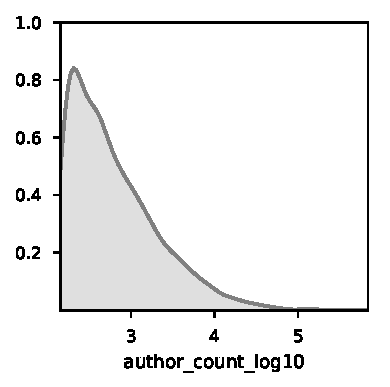
\includegraphics[width=\textwidth]{latex/kde/author_count_log10-active}
        \label{hist/sub:author}
    \end{subfigure}
    \hfill
    \begin{subfigure}[b]{0.49\textwidth}
        \centering
        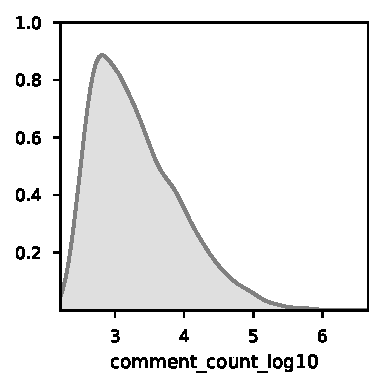
\includegraphics[width=\textwidth]{latex/kde/comment_count_log10-active.pdf}
        \label{hist/sub:comment}
    \end{subfigure}
    \hfill
    \begin{subfigure}[b]{0.49\textwidth}
        \centering
        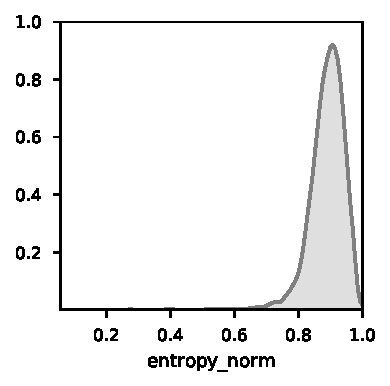
\includegraphics[width=\textwidth]{latex/kde/entropy_norm-active.pdf}
        \label{hist/sub:entropy}
    \end{subfigure}
    \hfill
    \begin{subfigure}[b]{0.49\textwidth}
        \centering
        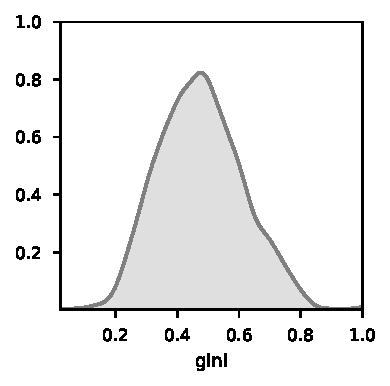
\includegraphics[width=\textwidth]{latex/kde/gini-active.pdf}
        \label{hist/sub:gini}
    \end{subfigure}
    \caption{Distributions of Subreddit-Level Statistics for Active Subreddit}
\end{figure} \label{hists/sub:active}
\begin{table}
\centering
\begin{tabular}{lrrrrrrr}
\toprule
{} &  entropy &  gini &  blau &  author\_count\_log10 &  comment\_count\_log10 &  entropy\_max &  entropy\_norm \\
\midrule
mean &    1.806 & 0.807 & 0.578 &               0.867 &                1.080 &        1.997 &         0.919 \\
std  &    1.817 & 0.212 & 0.380 &               0.881 &                1.047 &        2.029 &         0.102 \\
min  &    0.000 & 0.018 & 0.000 &               0.000 &                0.000 &        0.000 &         0.007 \\
25\%  &    0.000 & 0.655 & 0.000 &               0.000 &                0.301 &        0.000 &         0.892 \\
50\%  &    1.332 & 0.850 & 0.700 &               0.602 &                0.778 &        1.386 &         0.944 \\
75\%  &    2.797 & 1.000 & 0.920 &               1.342 &                1.653 &        3.091 &         0.986 \\
max  &   11.976 & 1.000 & 1.000 &               5.835 &                6.662 &       13.436 &         1.000 \\
\bottomrule
\end{tabular}
\caption{Descriptive Statistics for all Subreddits}
\label{table/all}
\end{table}
\begin{table}
\centering
\begin{tabular}{lrrrrrrr}
\toprule
{} &   mean &   std &   min &   25\% &    50\% &    75\% &    max \\
\midrule
author\_count\_log10  &  4.494 & 0.612 & 2.246 & 4.238 &  4.492 &  4.937 &  5.835 \\
blau                &  0.993 & 0.020 & 0.887 & 0.998 &  1.000 &  1.000 &  1.000 \\
comment\_count\_log10 &  4.878 & 0.671 & 2.650 & 4.526 &  4.858 &  5.306 &  6.662 \\
entropy             &  9.461 & 1.598 & 3.738 & 8.613 &  9.672 & 10.557 & 11.976 \\
entropy\_max         & 10.348 & 1.409 & 5.170 & 9.758 & 10.344 & 11.368 & 13.436 \\
entropy\_norm        &  0.910 & 0.064 & 0.712 & 0.901 &  0.934 &  0.946 &  0.983 \\
gini                &  0.511 & 0.101 & 0.278 & 0.459 &  0.517 &  0.577 &  0.801 \\
\bottomrule
\end{tabular}
\caption{Descriptive Statistics for Default Subreddits}
\label{table/defaults}
\end{table}
\begin{table}
\centering
\begin{tabular}{lrrrrrrr}
\toprule
{} &  mean &   std &   min &   25\% &   50\% &   75\% &    max \\
\midrule
entropy             & 5.724 & 1.138 & 0.318 & 4.913 & 5.493 & 6.325 & 11.976 \\
gini                & 0.476 & 0.137 & 0.021 & 0.378 & 0.471 & 0.567 &  1.000 \\
blau                & 0.986 & 0.034 & 0.070 & 0.986 & 0.992 & 0.996 &  1.000 \\
author\_count\_log10  & 2.798 & 0.524 & 2.158 & 2.377 & 2.667 & 3.089 &  5.835 \\
comment\_count\_log10 & 3.316 & 0.635 & 2.210 & 2.818 & 3.192 & 3.704 &  6.662 \\
entropy\_max         & 6.443 & 1.208 & 4.970 & 5.472 & 6.142 & 7.112 & 13.436 \\
entropy\_norm        & 0.889 & 0.062 & 0.056 & 0.862 & 0.897 & 0.927 &  1.000 \\
\bottomrule
\end{tabular}
\caption{Descriptive Statistics for Top Decile of Subreddits by Author Count}
\label{table/active}
\end{table}


\subsection{Subsetting Active Subreddits}
Table \ref{table/all} shows that at least half of subreddits had 3 or fewer unique comment authors in February 2018, and 4 or fewer comments. Both size measures are very highly skewed. I therefore decided to subset the top decile of subreddits by author count as 'active subreddits'.

Either one or both of \textit{author\_count} and \textit{comment\_count} could be used as a proxy for level of subreddit activity. In the full dataset the counts have a very strong positive correlation (coef = 0.899). 


\subsection{Findings}

As shown in Table \ref{table/active}, the lower quartile for \textit{blau} is 0.98. 90\% of the subsetted subreddits have a blau value greater than or equal to 0.96.  Thus, \textit{blau} does not appear to be an informative measure for general trends in active subreddits. However it may still be of use to look into the lower extremes for \textit{blau}. Table \ref{table/active} shows \textit{blau} has a minimum value of 0.078. This outlier way provide insight.

\textcolor{red}{Refer to \ref{blau index} to determine whether the blau index should be normalised.}

Figure \ref{hists/sub:active} shows the distributions for \textit{normalised entropy} and \textit{gini}. Both are normally distributed. Table \ref{table/active} shows that \textit{entropy\_norm} has quartiles Q1 = 0.846, Q2 = 0.883, Q3 = 0.914 and mean 0.873. An average normalised entropy for active subreddits it ~0.87/8. Section \ref{entropy} showed that the higher a subreddit's entropy, the greater it's diversity. As normalised entropy has an upper limit of 1, the average of 0.8 shows that most subreddits have high diversity in terms of the range of authors commenting in the subreddit.

The same table shows that \textit{blau} has quartiles Q1 = 0.363, Q2 = 0.455, Q3 = 0.547 and mean 0.458. An average \textit{gini} for active subreddits it ~0.45. Section \ref{gini} showed that a gini coefficient of 0 means perfect equality, and 1 means perfect inequality. An average of 0.45 therefore suggests that active subreddits tend to have a mid-level of equality.

Normalised entropy and gini have a Pearson correlation coefficient of 0.771 and a Spearman's rank correlation coefficient of 0.898. The measures of diversity are highly positively correlated. It may be of interest to determine the for which subreddits they are not highly correlated, and why. This would help understand the relationship between the measures and how to interpret their different magnitudes. Active subreddits are highly diverse, as measured by entropy but neither inequal or equal, as measured by gini.